\chapter{Evaluation}
\label{chp:chapter_4}
The evaluation of our system is split up in a \textit{static} and a \textit{dynamic} part. The static evaluation quantifies the connection setup performance for each optimization stage. The static behavior will be benchmarked on \textit{number of packets during connection setup}, \textit{connection setup time}, \textit{connection parameter update time}, \textit{time until first useful packet}, and \textit{power consumption}. The dynamic evaluation is about quantifying the performance of FRAPPUCcInO, which will be based on \textit{average throughput}, and \textit{responsiveness}.

This separation is made because the static performance improvement will be applicable to both intermittently-powered and conventionally-powered devices. Reducing connection setup time and power consumption on their own are attractive propositions since it improves responsiveness and battery life. The FRAPPUCcInO algorithm is not the only possible application of \textit{Fast Reconnect}. For example, Fast Reconnect could also be leveraged to quickly build a connection when ambient energy is insufficient for even the maximum connection interval, allowing a pseudo-connected state. 

\section{Experimental Setup}
\label{sec:evaluation_setup}
The demo application described in Section \ref{sec:demo_application} was also used for all experiments. The central is an nRF52840DK development board, and the peripheral is the modified FreeBie platform. The nRF52840-Dongle was used as a sniffer for Wireshark. During the static testing, the Nordic Power Profiler Kit II (PPK-II) was used to power FreeBie and measure its power consumption. During the dynamic testing, the PPK-II was replaced with a 46.5$\mu\text{W}$ solar cell from Panasonic \cite{panasonic_solar}, and a Saleae Logic Pro 8 was used to capture digital and analog traces \cite{saleae_logic_pro_8}. Finally, an Ikea TRÅDFRI smartlight was calibrated and controlled through \texttt{python} to simulate changing energy harvesting conditions. 

The \texttt{CMakeLists} file has been retrofitted to enable easy switching between optimization stages during testing. Set the \texttt{CMake} variables according to Table \ref{tbl:stage_defs} to enable a specific stage.
\begin{table}
    \begin{center}
    \begin{tabular}{|l|l|l|l|l|}
        \hline
                                & \multicolumn{4}{c|}{\textbf{Stage}}   \\
        \textbf{Variable}    & \textbf{1} & \textbf{2} & \textbf{3} & \textbf{4} \\
        \hline
        CACHE\_SERVICE\_DISCOVERY &   & 1 & 1 & 1 \\
        \hline
        SKIP\_RECONF             &   &   & 1 & 1 \\
        \hline
        CACHE\_LL\_FEAT\_EXCH      &   &   &   & 1 \\
        \hline
        CACHE\_LL\_DL\_EXCH        &   &   &   & 1 \\
        \hline
    \end{tabular}
    \end{center}
    \caption{\texttt{CMake} variables to set for a given optimization stage. Set the variable to 1 if the cell contains a 1, otherwise do not set the variable.}
    \label{tbl:stage_defs}
\end{table}

\section{Results}
\label{sec:evaluation_results}

\subsection{Static}
\label{sec:static_evaluation}
% Number of Packets Plot
\begin{figure}[]
    \centering
    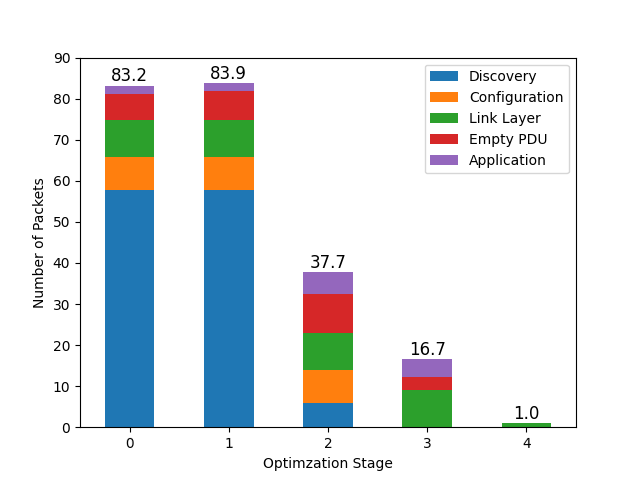
\includegraphics[width=0.5\textwidth,height=6cm,keepaspectratio=true]{plots/static_packet_division.png}
    \caption{
        Number of packets from the \texttt{CONNECT\_IND} up to the last connection setup packet.
    }
    \label{fig:static_packet_division}
\end{figure}

When at the number of packets sent between the \texttt{CONNECT\_IND} packet and the first packet that does not belong to the connection setup, shown in Figure \ref{fig:static_packet_division}, a significant reduction can be seen. From Stage 0 (no modifications) to Stage 4 (all modifications) this is a reduction of \textbf{98.80\%}. When only sharing the preferred (slower) connection parameters (Stage 1), the average number of packets goes up by 0.7 packets. This increase in packets is a result of slighty more Empty PDUs being as a result of different timing. Stage 2 still counts 6 packets for \textit{discovery}, even though service discovery caching is being used, because reading the Database Hash requires 3 packets for both the central and peripheral. 

% Setup Time Plot
\begin{figure}[]
    \centering
    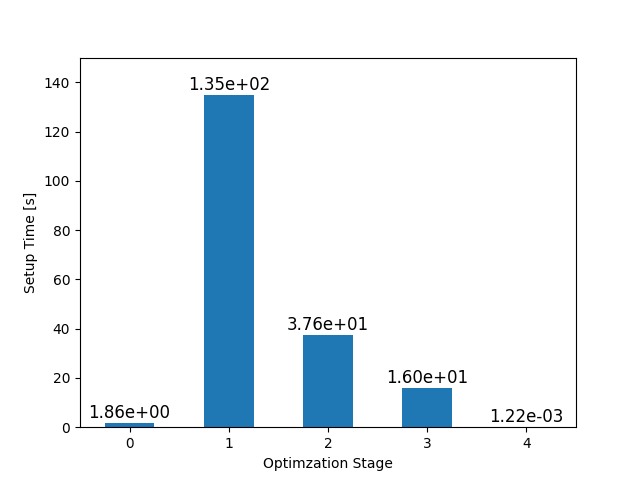
\includegraphics[width=0.5\textwidth,height=6cm,keepaspectratio=true]{plots/static_setup_time.png}
    \caption{
        Connection setup time, measured from \texttt{CONNECT\_IND} up to the last packet that does not belong to the connection setup.
    }
    \label{fig:static_setup_time}
\end{figure}

Figure \ref{fig:static_setup_time} shows the time required to setup a connection, measured from \texttt{CONNECT\_IND} up to the last packet that does not belong to the connection. At first, Stage 1 through 3 seem significantly worse than stage 0. However, it is important to remember that in Stage 0, the peripheral is forced to use the default connection parameters of the central. As a result, our system needs to be designed with a much larger capacitor than required after the connection is established. Although slower, Stage 1 allows us to reduce the size of the capacitors used in our system, which allows the system to recover much faster after a full power failure, as well as reducing the systems overal size and cost. Stage 4 reduces the connection setup to a single packet, resulting in a reduction of \textbf{99.93\%}.

% Time To Useful Packet Plot
\begin{figure}[]
    \centering
    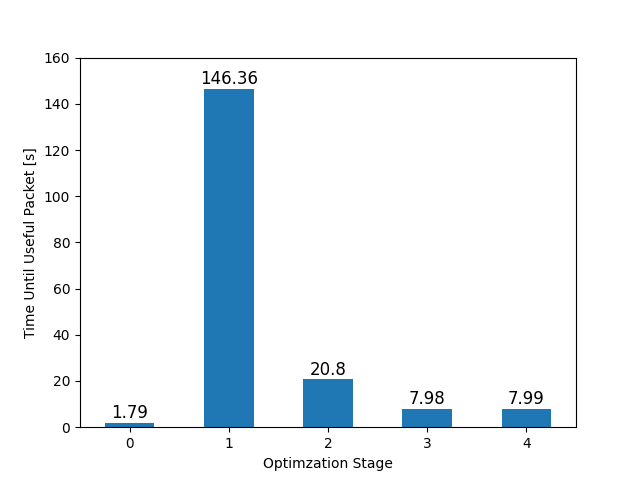
\includegraphics[width=0.5\textwidth,height=6cm,keepaspectratio=true]{plots/static_useful_packet_time.png}
    \caption{
        Time until first useful packet. Measured from \texttt{CONNECT\_IND} up to the first useful application packet.
    }
    \label{fig:static_useful_packet_time}
\end{figure}

To measure the fastest possible time until a useful packet is received by the central, we perform a \textit{Read Request} from the central on the \textit{battery level} characteristic. A \textit{useful packet} is defined as anything that directly contributes to the function of an application. For example, a read or write request on a characteristic, or a write request on a CCC to enable Notifications. 

From Figure \ref{fig:static_useful_packet_time} one can see that Stage 4 is about 4.46 times slower than Stage 0. However, the default connection interval used by Zephyr in Stage 0 is 50 milliseconds, which is 80 times slower than the connection interval used by Stage 4. The iprovements in Stages 2, 3, and 4 are able to recoup a significant amount of the time gained by using the slowest connection parameters, which is visible from Stage 1 in Figure \ref{fig:static_useful_packet_time}. It is also notable that eight seconds is the lower limit that is possible at a connection interval of four seconds, since a complete read operation from a GATT server requires two packets. The fact that there is no decrease from Stage 3 to Stage 4 is supported by the idea that the link layer procedures 

% Connection Adaption Time vs. current CI
\begin{figure}[]
    \centering
    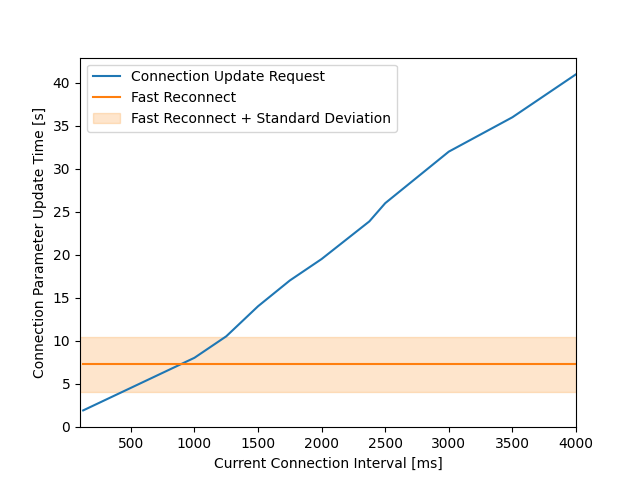
\includegraphics[width=0.5\textwidth,height=6cm,keepaspectratio=true]{plots/static_conn_update_plot.png}
    \caption{
        Time until new connection parameters are applied versus currently used connection parameters.
    }
    \label{fig:static_conn_update_time}
\end{figure}

Figure \ref{fig:static_conn_update_time} shows the time it takes for new connection parameters to be applied when using the regular \textit{connection update request} versus \textit{Fast Reconnect}. Since the time required to reconnect using fast reconnect is independent of connection interval, the time to update connection parameters does not increase as connection interval increases. However, fast reconnect is more variable since it requires the central to receive a new advertisement from the peripheral. One standard deviation is shown in Figure \ref{fig:static_conn_update_time} with light orange. An optimal approach would use the conventional connection update request when CI is below 1250, and fast reconnect for CI above 1250.

% Energy Used vs. Optimzation Stage
\begin{figure}[]
    \centering
    \begin{minipage}[b]{0.47\textwidth}
      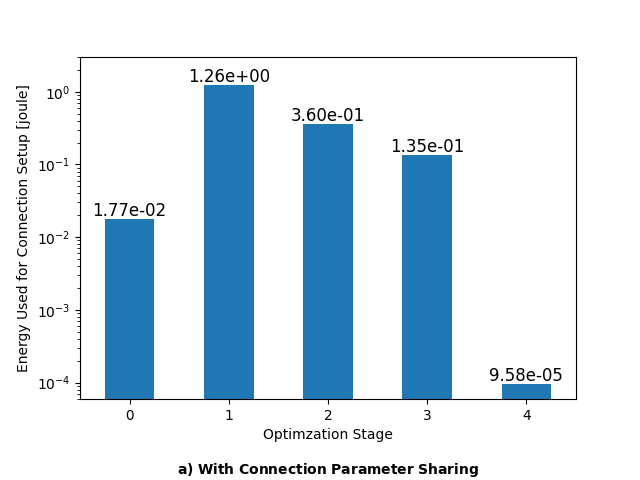
\includegraphics[width=\textwidth]{plots/static_power_consumption_conventional.png}
    \end{minipage}
    \hfill
    \begin{minipage}[b]{0.47\textwidth}
        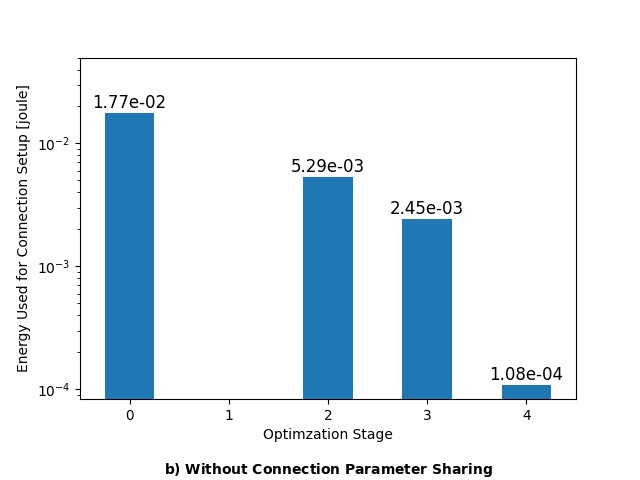
\includegraphics[width=\textwidth]{plots/static_power_consumption_conventional_fast.png}
    \end{minipage}
    \caption{Energy consumed (in Joule) during connection setup versus optimization stage when continuously-powered. a) Uses Connection Parameter Sharing (Stage 1). b) Does not use Connection Parameter Sharing.}
    \label{fig:static_power_consumption_conventional}
\end{figure}

As one can see in Figure \ref{fig:static_power_consumption_conventional}a, when continuously-powered and using slow connection parameters, the total energy consumed only drops below Stage 0 when using all optimzations. This is because the microcontroller is still using power while idling, so extending the setup time by increasing the connection interval will cause higher energy usage. However, when using all optimzations, the energy usage is \textbf{reduced by 99.46\%}. When using these optimizations in devices that do not employ energy harvesting, it is adviced to reduce the connection parameters after the setup process is done. This is shown in Figure \ref{fig:static_power_consumption_conventional}b.

\begin{figure}[]
    \centering
    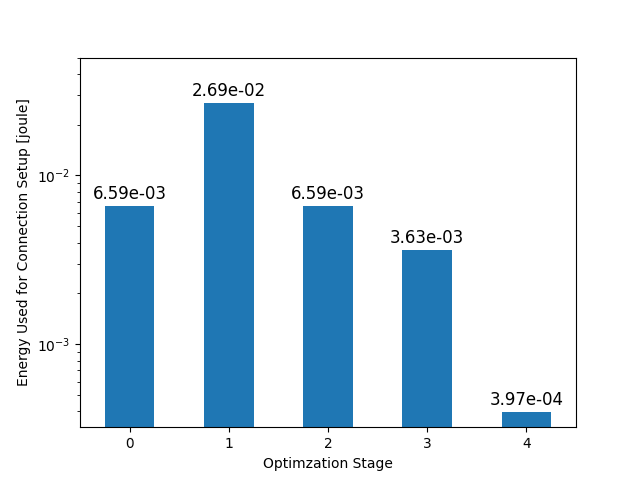
\includegraphics[width=0.5\textwidth,height=6cm,keepaspectratio=true]{plots/static_power_consumption_intermittent.png}
    \caption{
        Energy consumed (in Joule) during connection setup versus optimization stage when intermittently-powered. 
    }
    \label{fig:static_power_consumption_intermittent}
\end{figure}

Figure \ref{fig:static_power_consumption_intermittent} shows the energy used during the connection setup while intermittently-powered. Stage 3 and 4 show a significant reduction in energy consumed with \textbf{44.96\%} and \textbf{93.97\%}, respectively. However, Stage 1 and 2 might still be an improvement when intermittently-powered, since the average current draw during connection setup is 68.96$\mu$A, and 71.13$\mu$A, compared to 1.21mA of Stage 0. This reduced continuous current draw might allow an intermittently-powered device to remain operational using Stage 1, while Stage 0 would result in the capacitor voltage becoming critically low.

\subsection{Dynamic}
\label{sec:dynamic_evaluation}
\begin{figure}[]
    \centering
    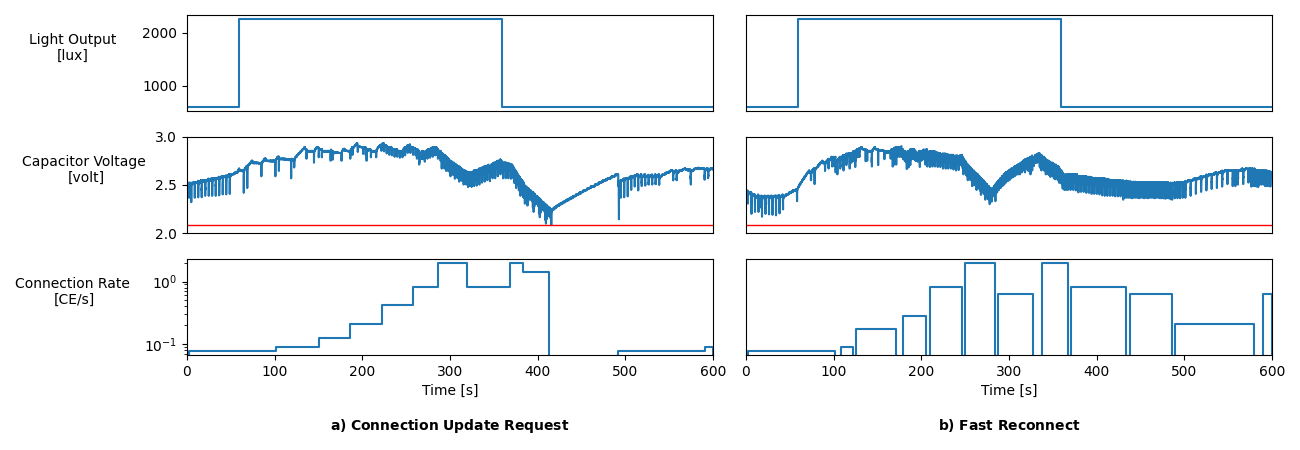
\includegraphics[width=1\textwidth,height=6cm,keepaspectratio=true]{plots/dynamic_short_both.png}
    \caption{
        Connection Rate versus Light Output
    }
    \label{fig:dynamic_short_both}
\end{figure}

Figure \ref{fig:dynamic_long_both} shows an optimal situation for using FRAPPUCcIno, which is a sharp increase followed by a sharp decrease in available power after using slow connection parameters. In this scenario, using Fast Reconnect allows an earlier rise, as well as allowing the system to respond in time to prevent a power failure. As a result, FRAPPUCcInO using Fast Reconnect is able to maintain an average throughput of \textbf{24.29\%} higher when compared to FRAPPUCcInO using the regular Connection Update Request. We define the responsiveness as the peak-to-peak time between the \textit{light output} and the \textit{connection rate}. Using this definition, FRAPPUCcInO with Fast reconnect reaches its peak 191 seconds after the light ouput rises, and FRAPPUCcInO using Connection Update Request reaches its peak after 227 seconds. The responsiveness is therefore improved by \textbf{15.86\%}.


\begin{figure}[]
    \centering
    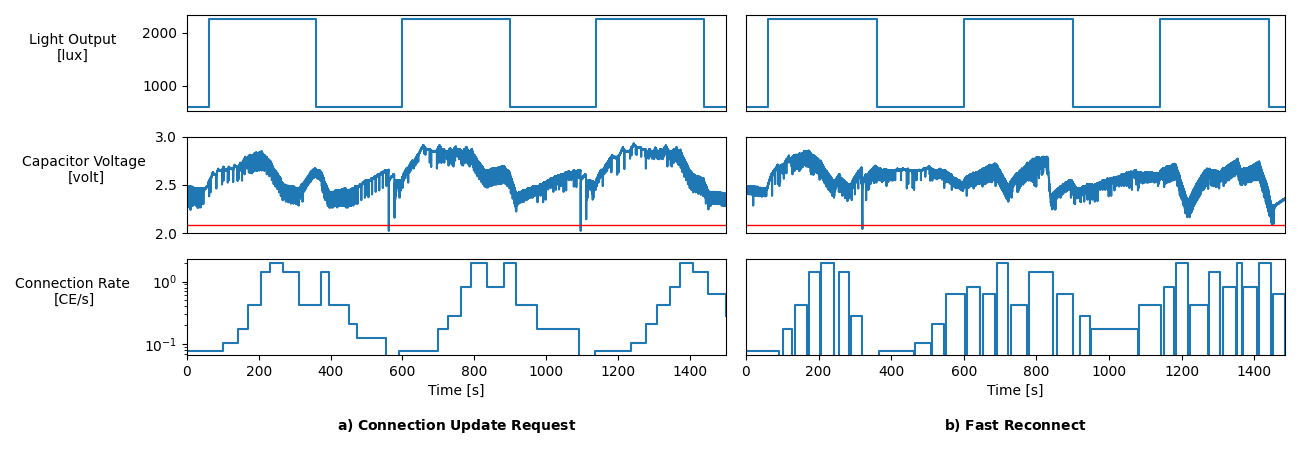
\includegraphics[width=1\textwidth,height=6cm,keepaspectratio=true]{plots/dynamic_long_both.png}
    \caption{
        Connection Rate versus Light Output. \textbf{left}) Connection Update Request. \textbf{right}) Fast Reconnect.
    }
    \label{fig:dynamic_long_both}
\end{figure}

When performing a long run, the advantage in throughput is less drastic but still significant. Figure \ref{fig:dynamic_long_both} shows a 25 minute run with multiple peaks in light output. In this scenario, the average throughput is \textbf{10.87\%} higher for FRAPPUCcInO using Fast Reconnect. However, responsiveness has improved by \textbf{107\%}. This improvement can be attributed to the fact that FRAPPUCcInO with Fast Reconnect is able to decrease the throughput earlier to start charging the capacitor up. As a result, FRAPPUCcInO reaches the voltage where it can increase the throughput again much earlier. We should note that during runs longer than 15 minutes, both systems were very like to encounter hard faults. These instability issues should be fixed before we are able to fully assess the performance of FRAPPUCcInO over longer periods.